\documentclass{article}
\usepackage{graphicx}
\usepackage{float}

\author{Austin Chase Minor}
\date{\today}
\title{Programing Project}

\begin{document}
\begin{enumerate}
\item 
  Algorithm 1
  \begin{figure}[H]
    \centering
    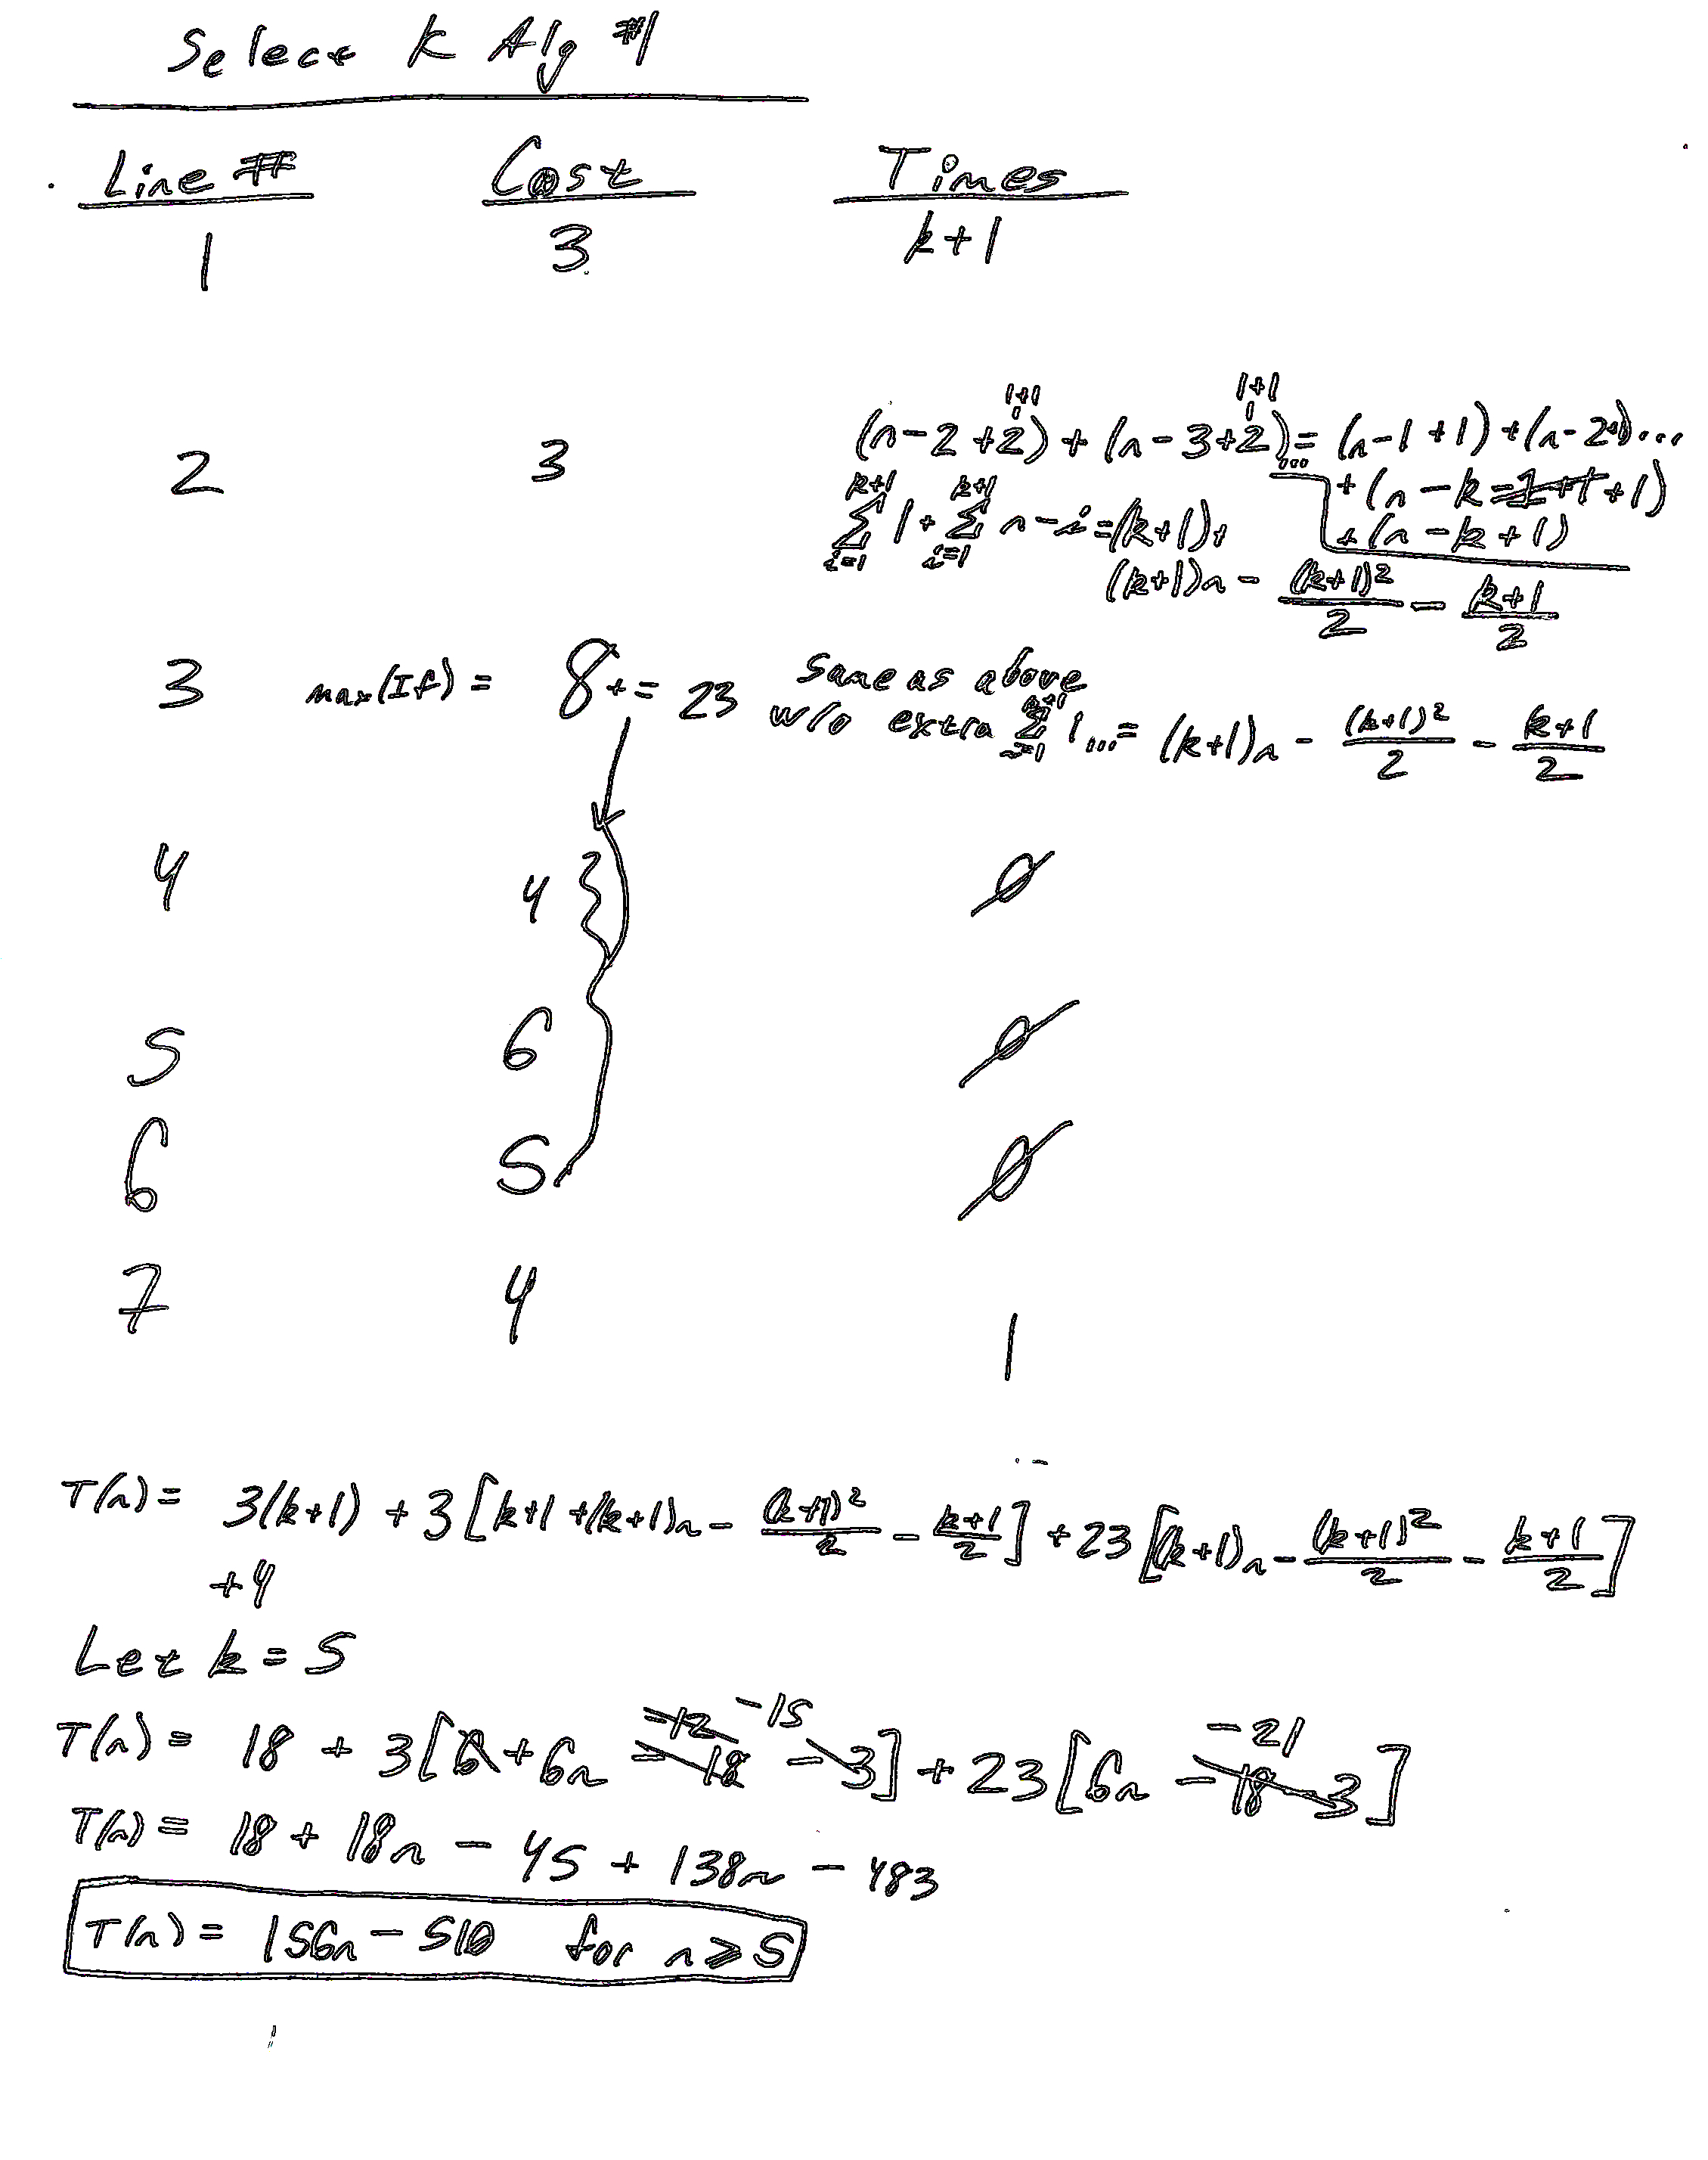
\includegraphics[width = \textwidth]{pics/alg1}
  \end{figure}

  Algorithm 2
  \begin{figure}[H]
    \centering
    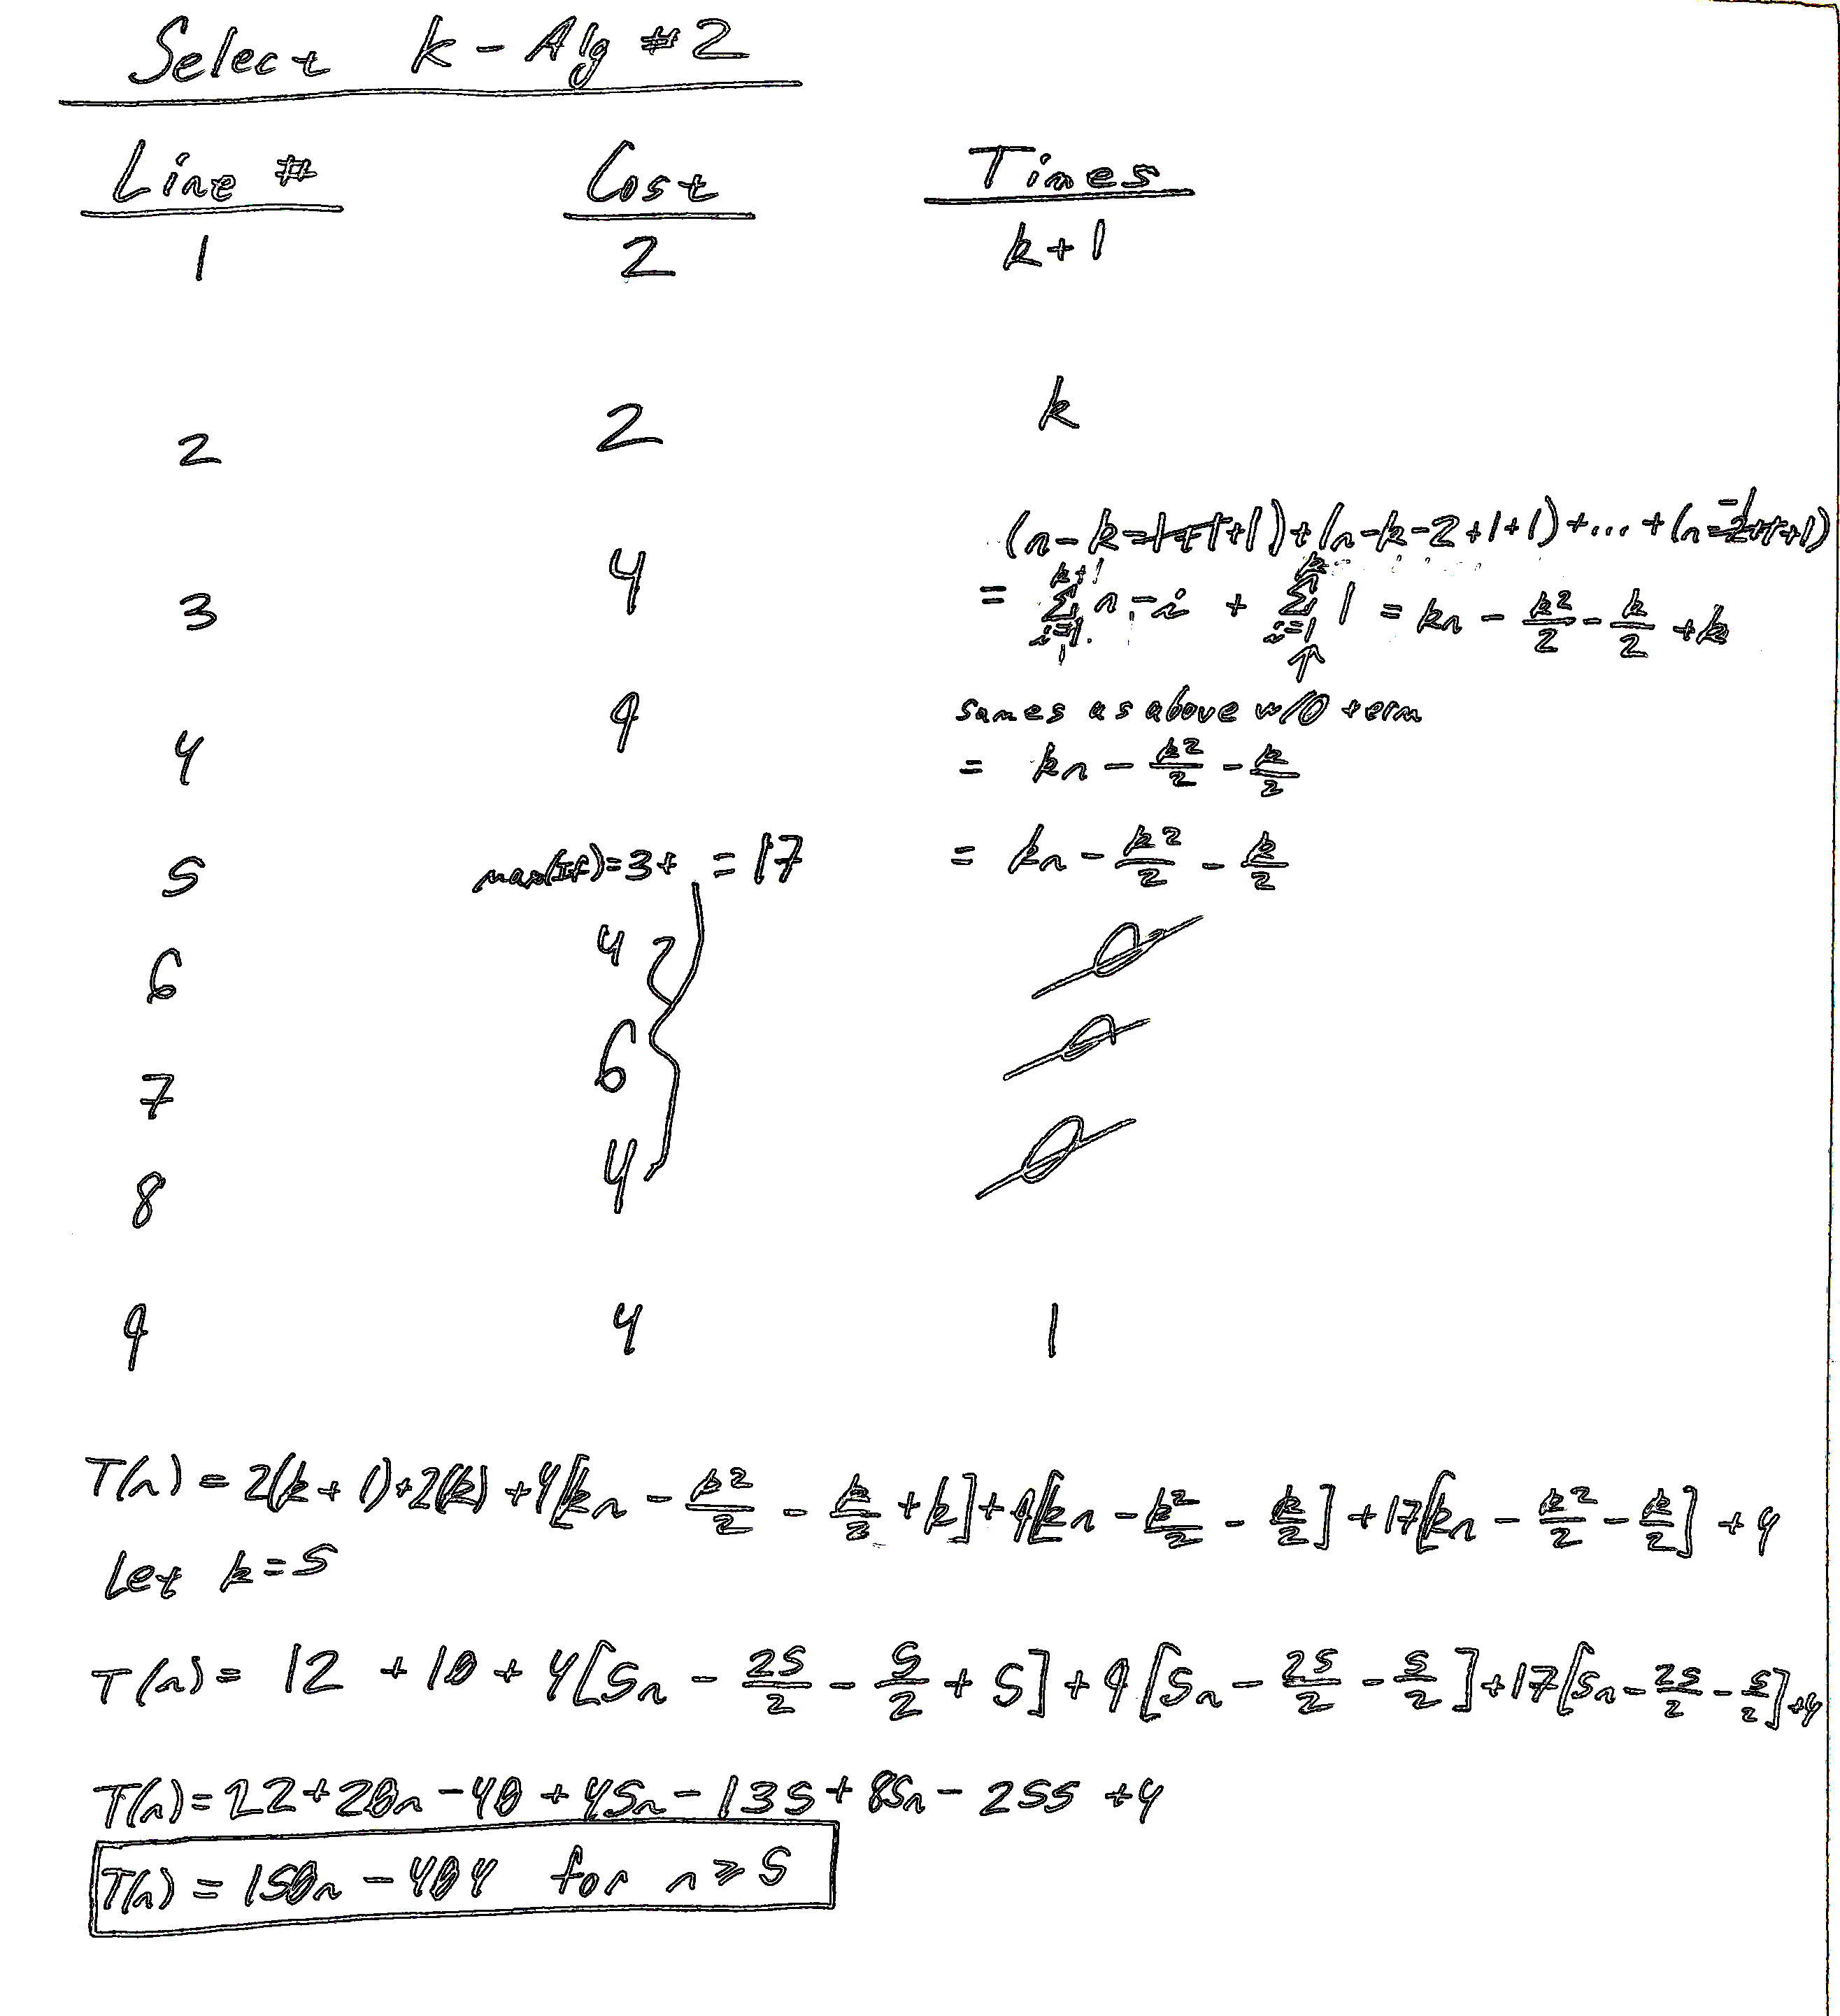
\includegraphics[width = \textwidth]{pics/alg2}
  \end{figure}

  Algorithm 3
  \begin{figure}[H]
    \centering
    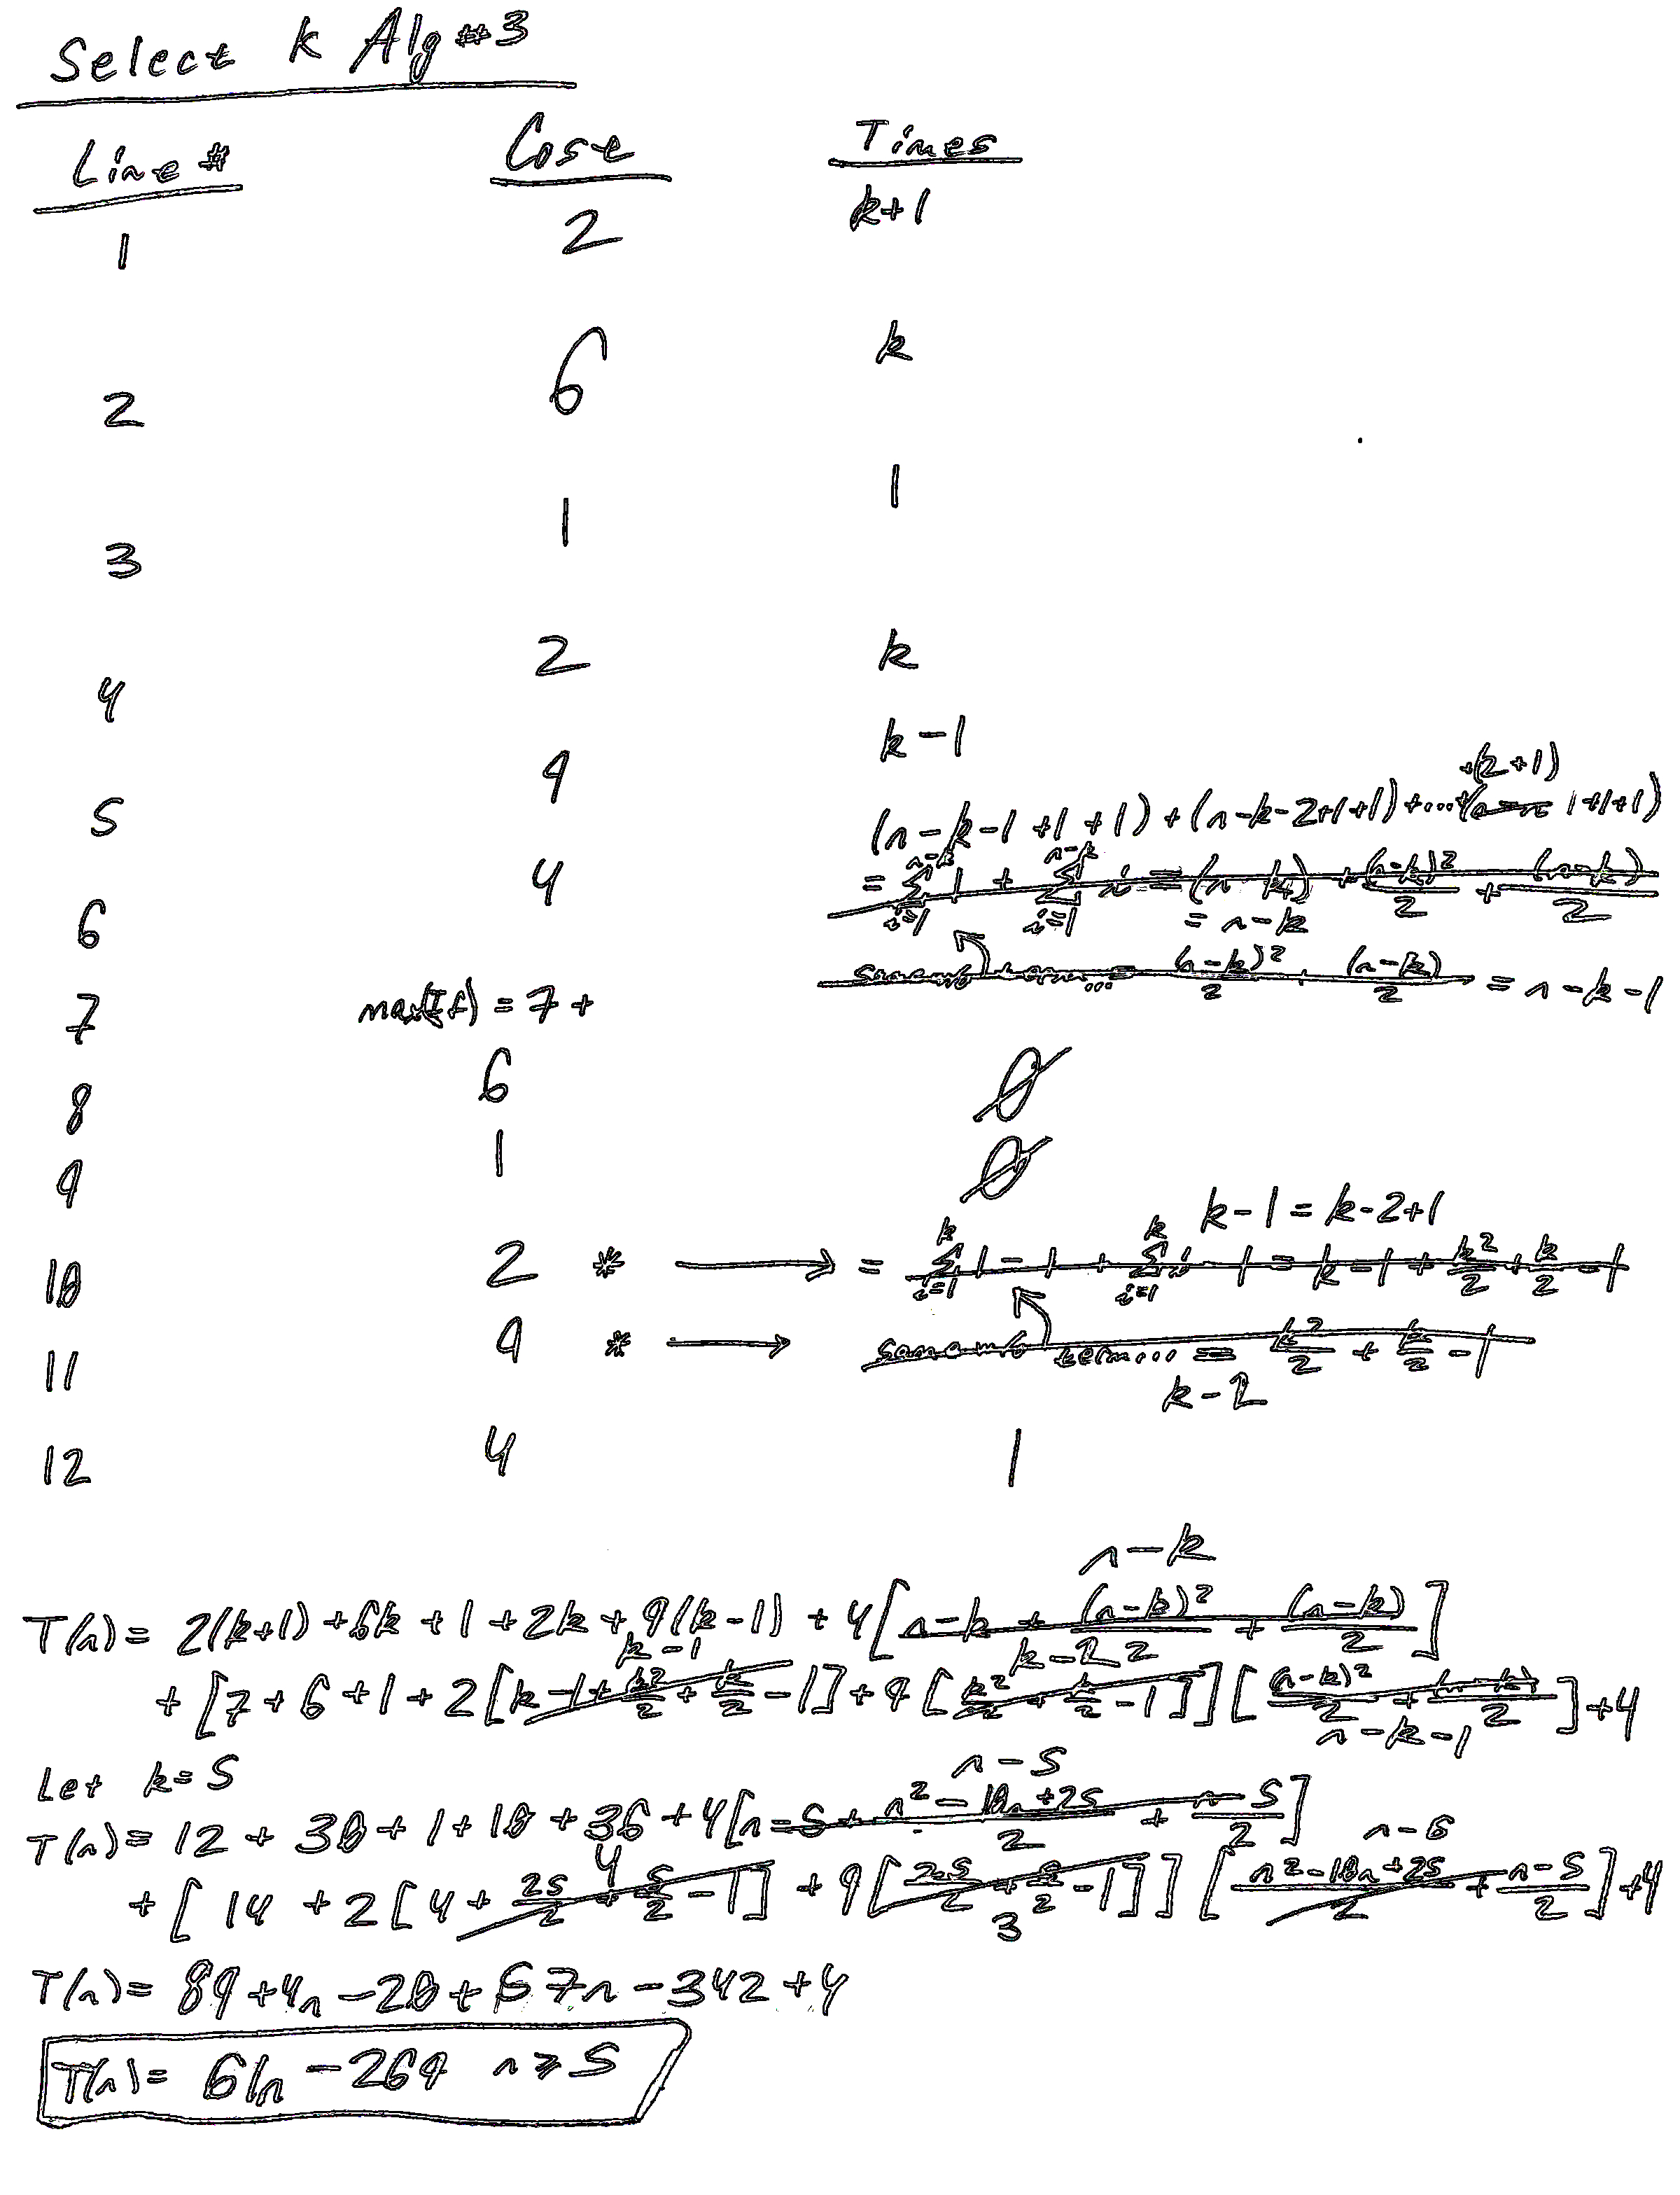
\includegraphics[width = \textwidth]{pics/alg3}
  \end{figure}

  Algorithm 4
  \begin{figure}[H]
    \centering
    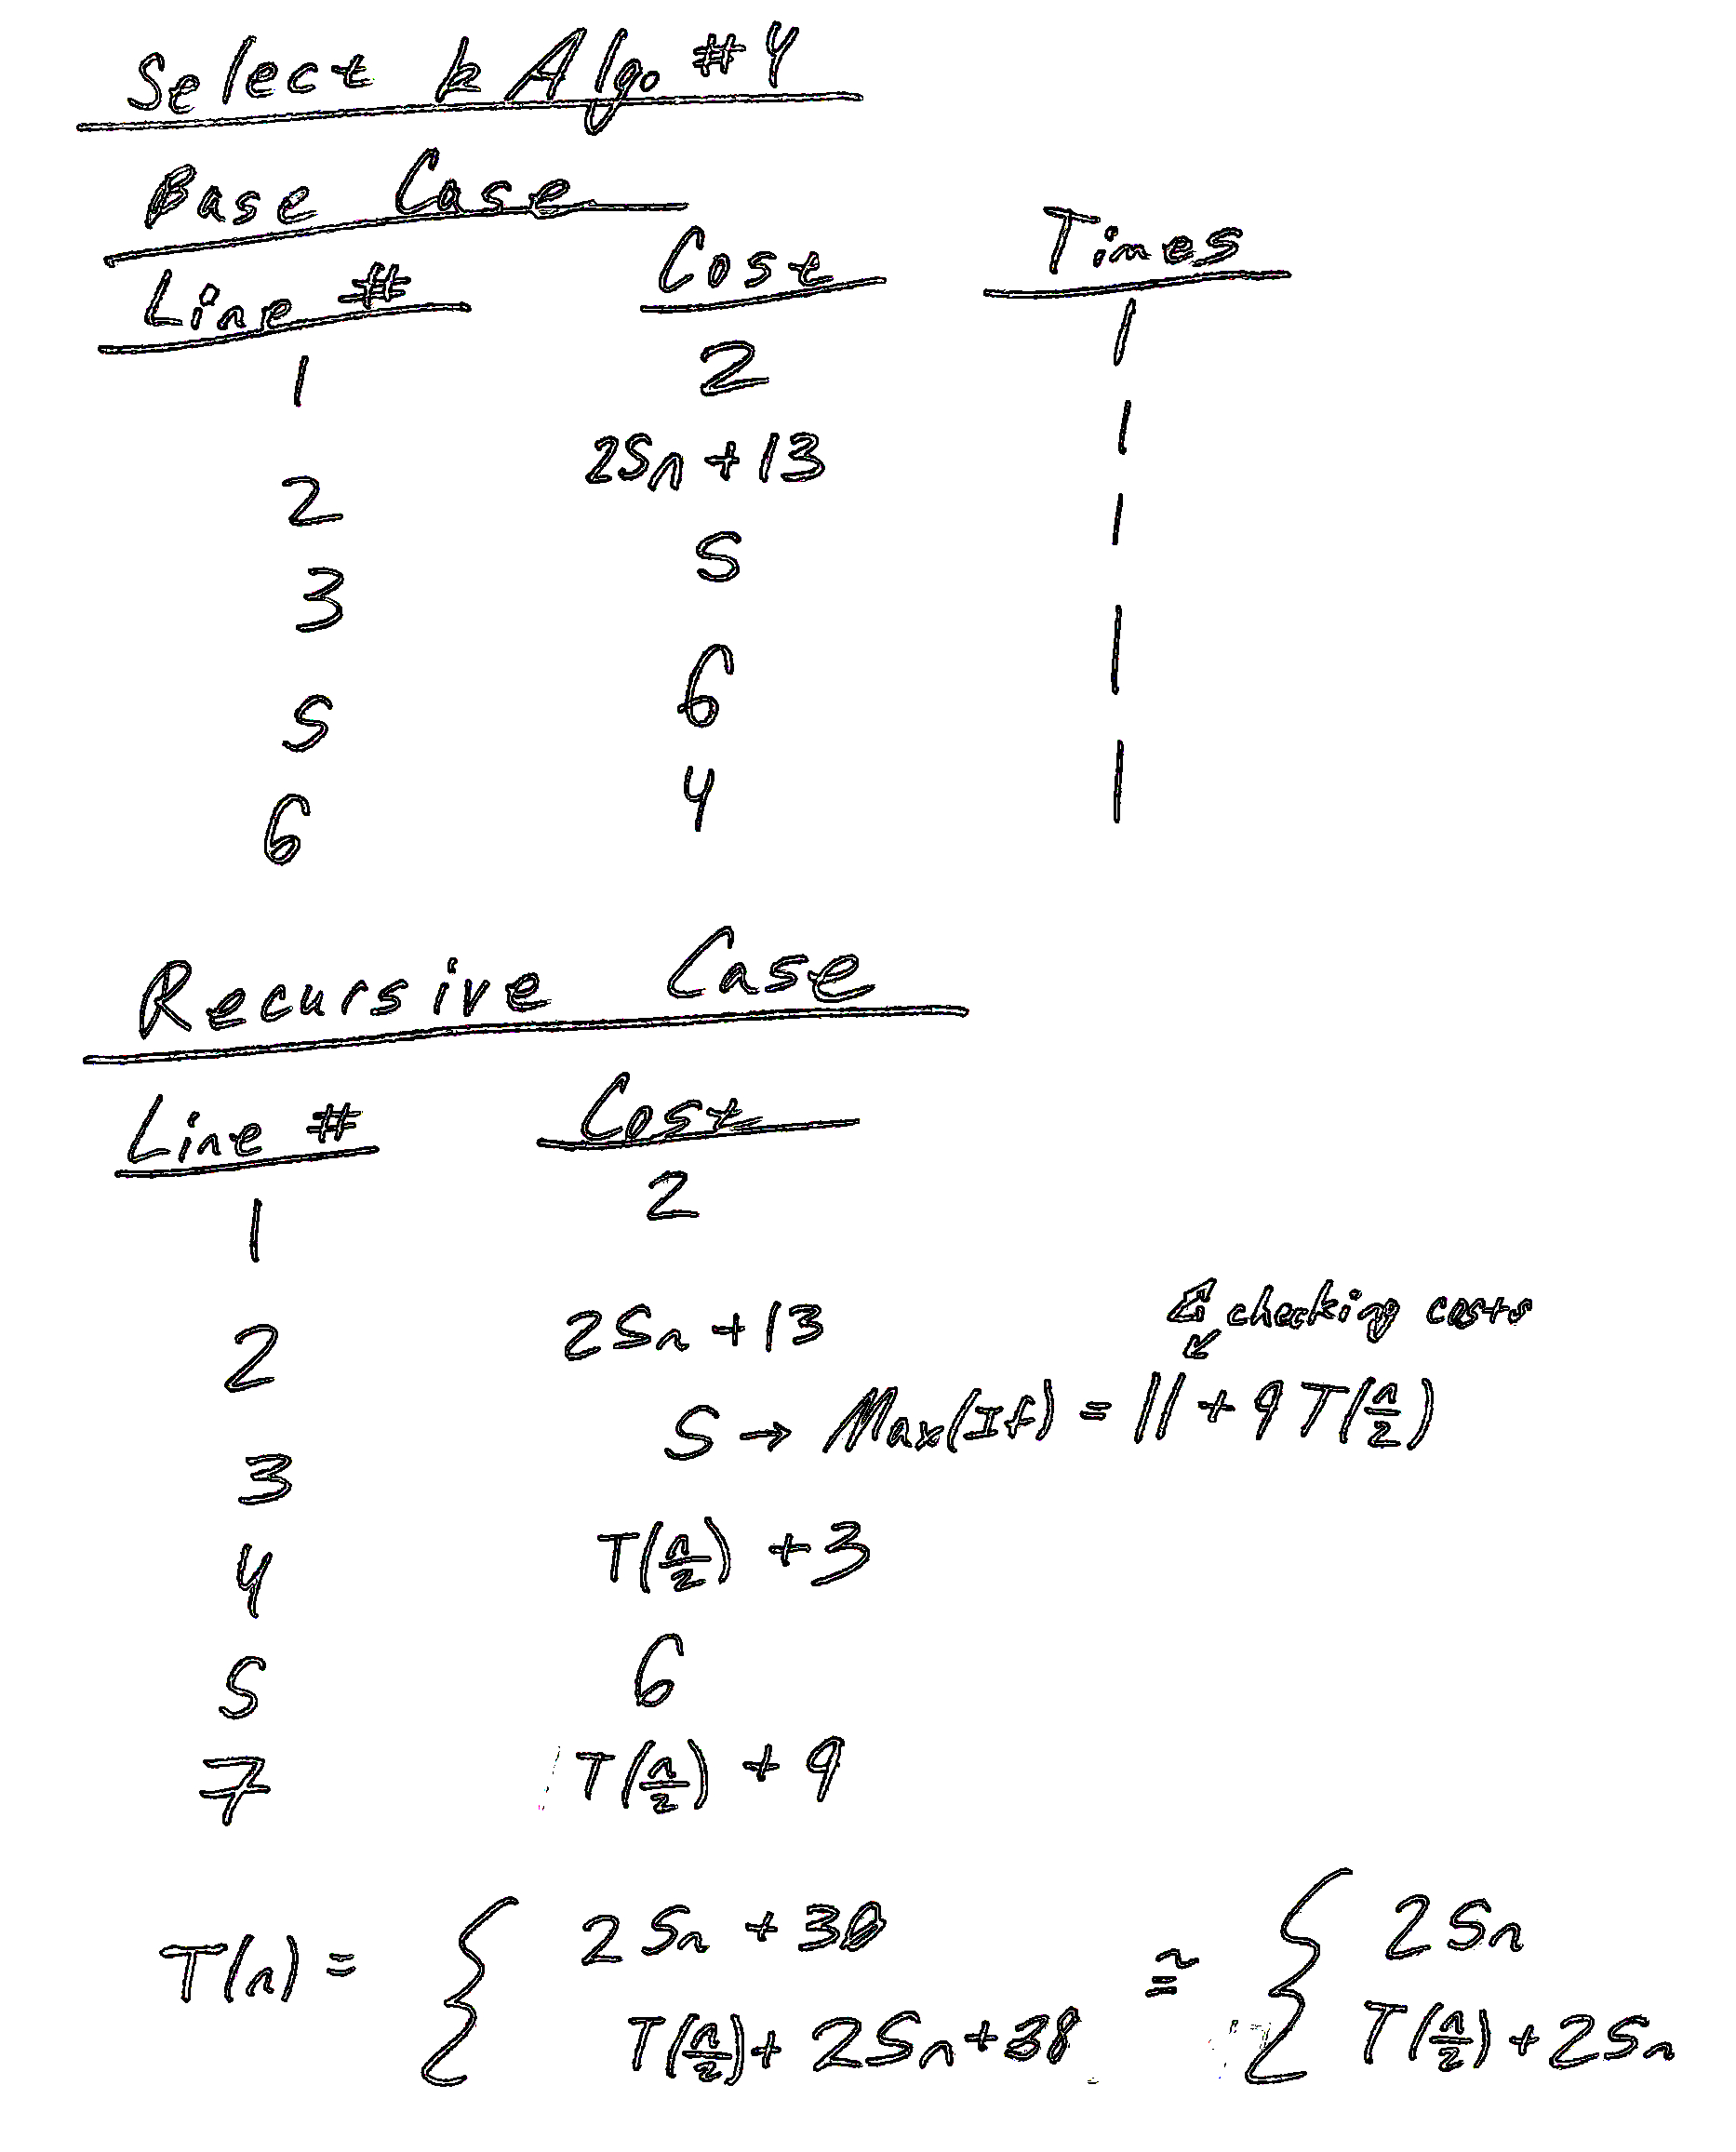
\includegraphics[width = \textwidth]{pics/alg4a}
  \end{figure}
  \begin{figure}[H]
    \centering
    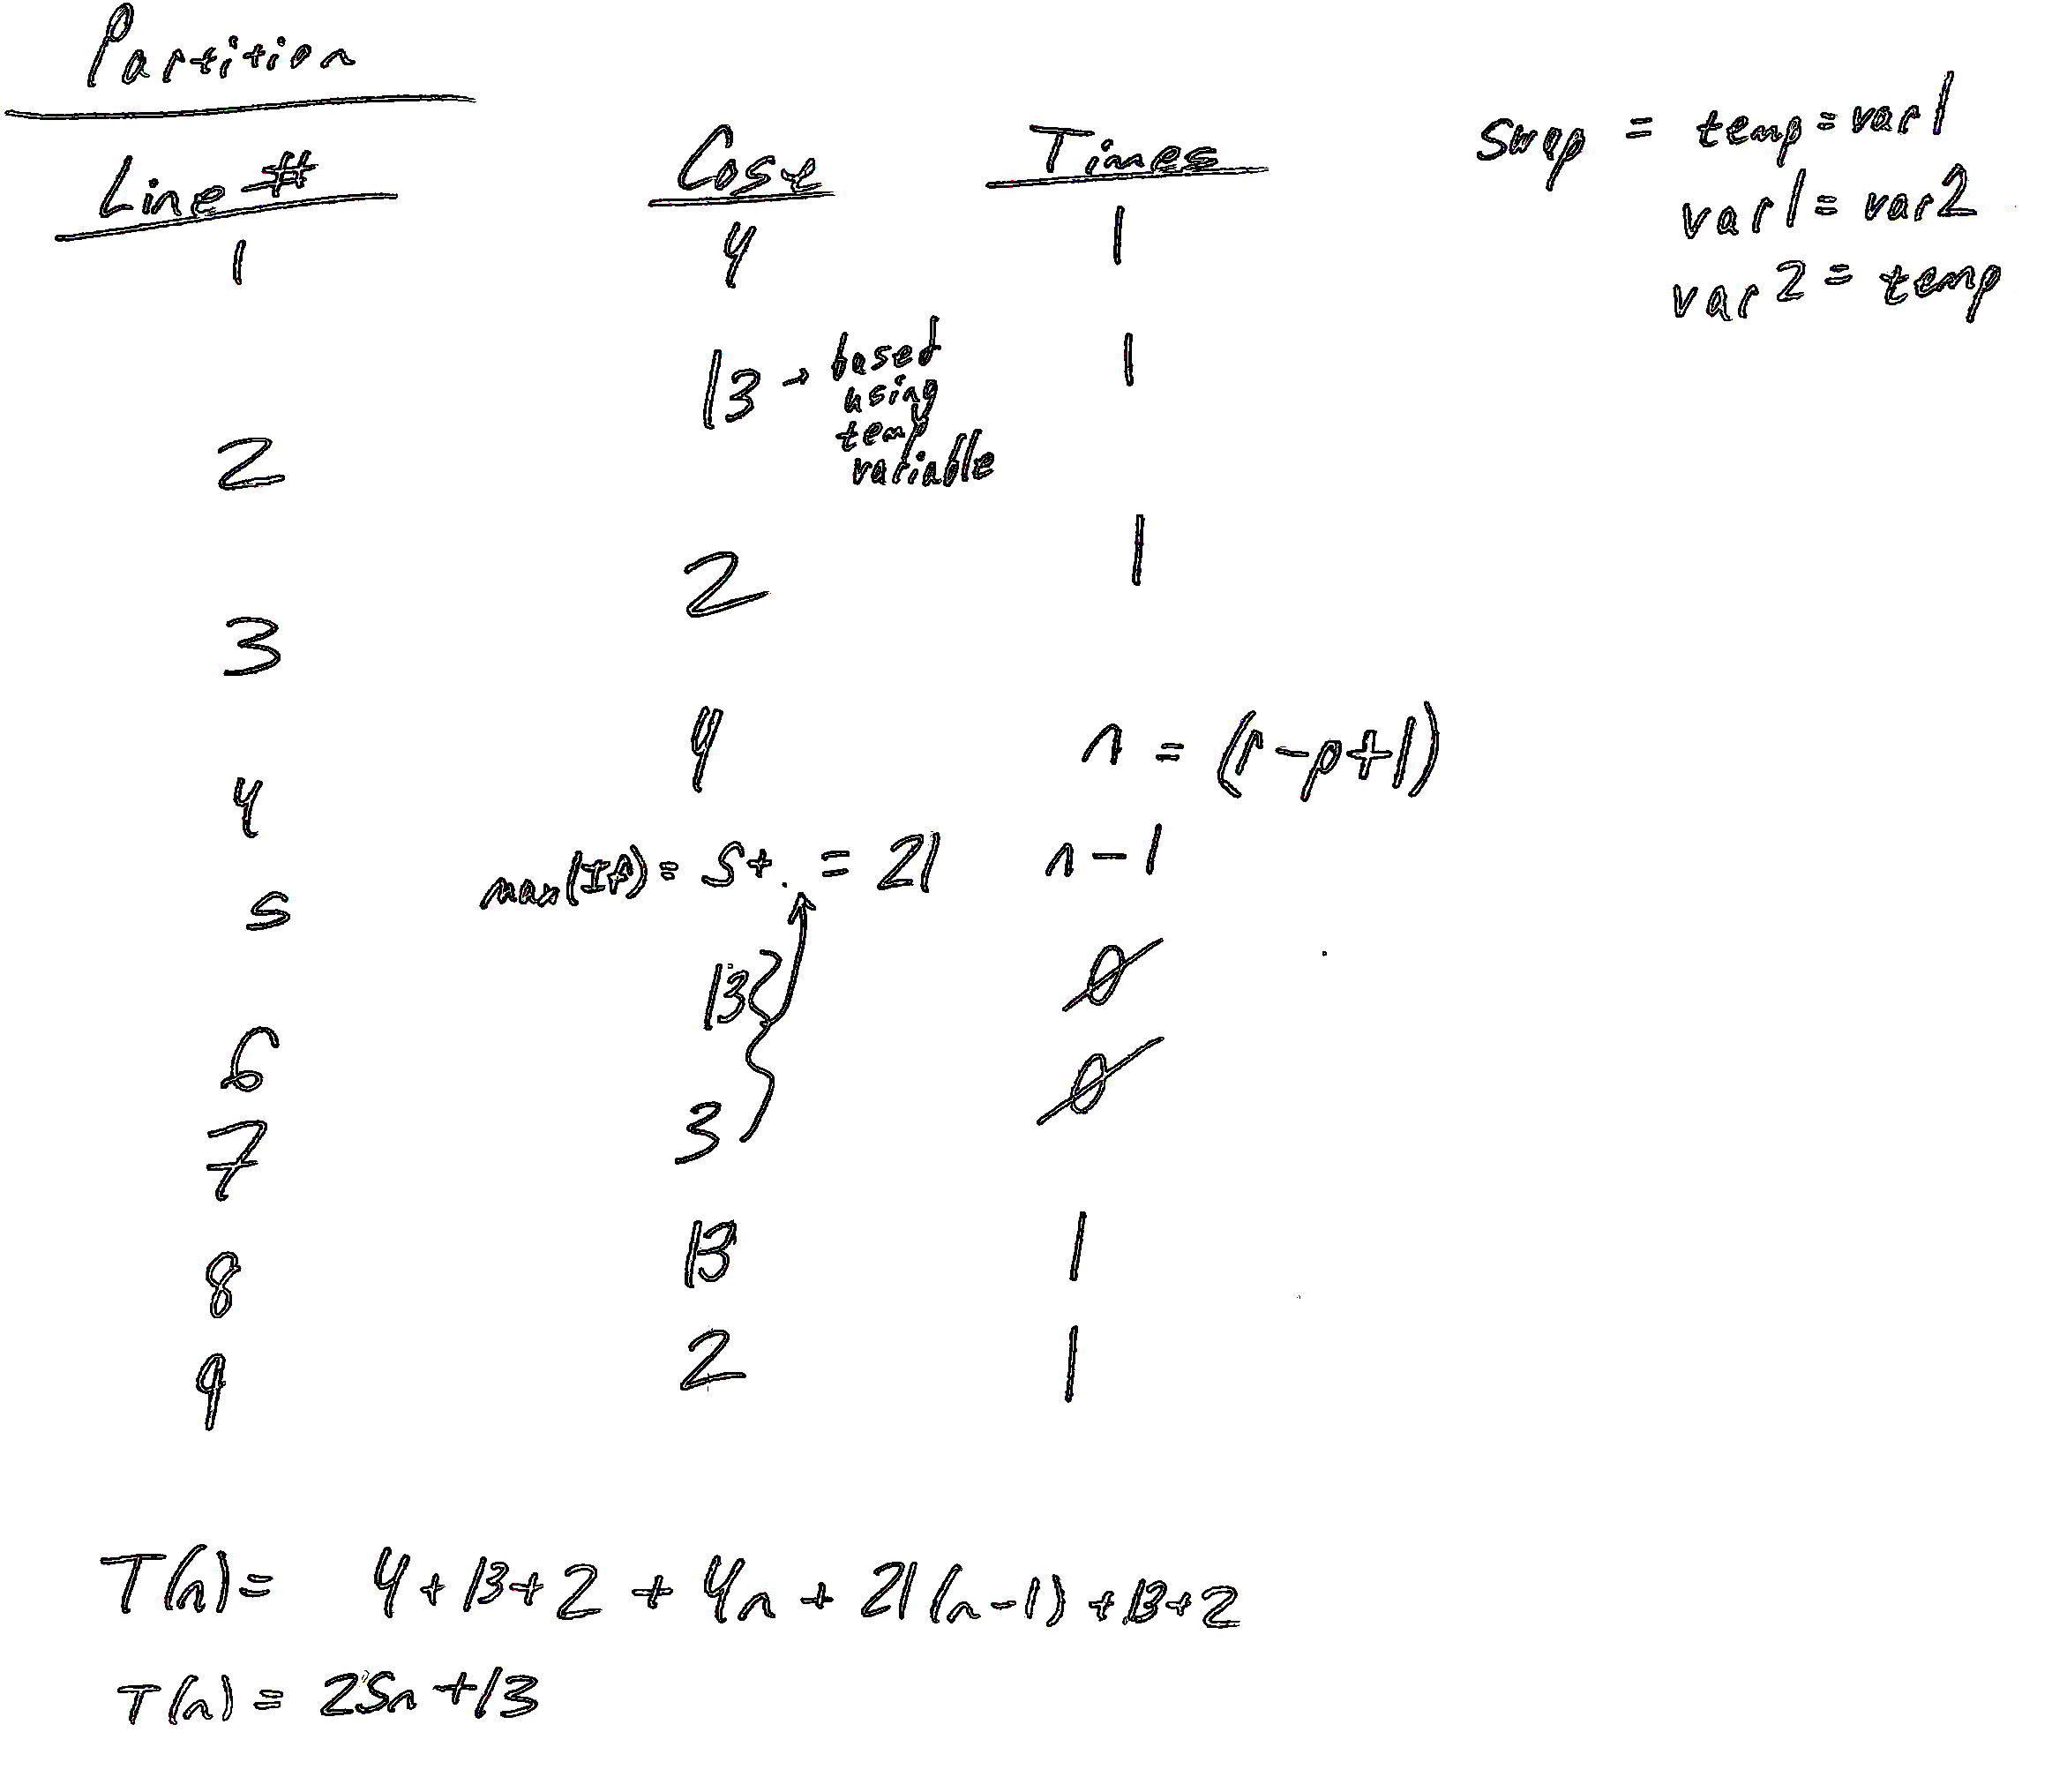
\includegraphics[width = \textwidth]{pics/alg4b}
  \end{figure}
  \begin{figure}[H]
    \centering
    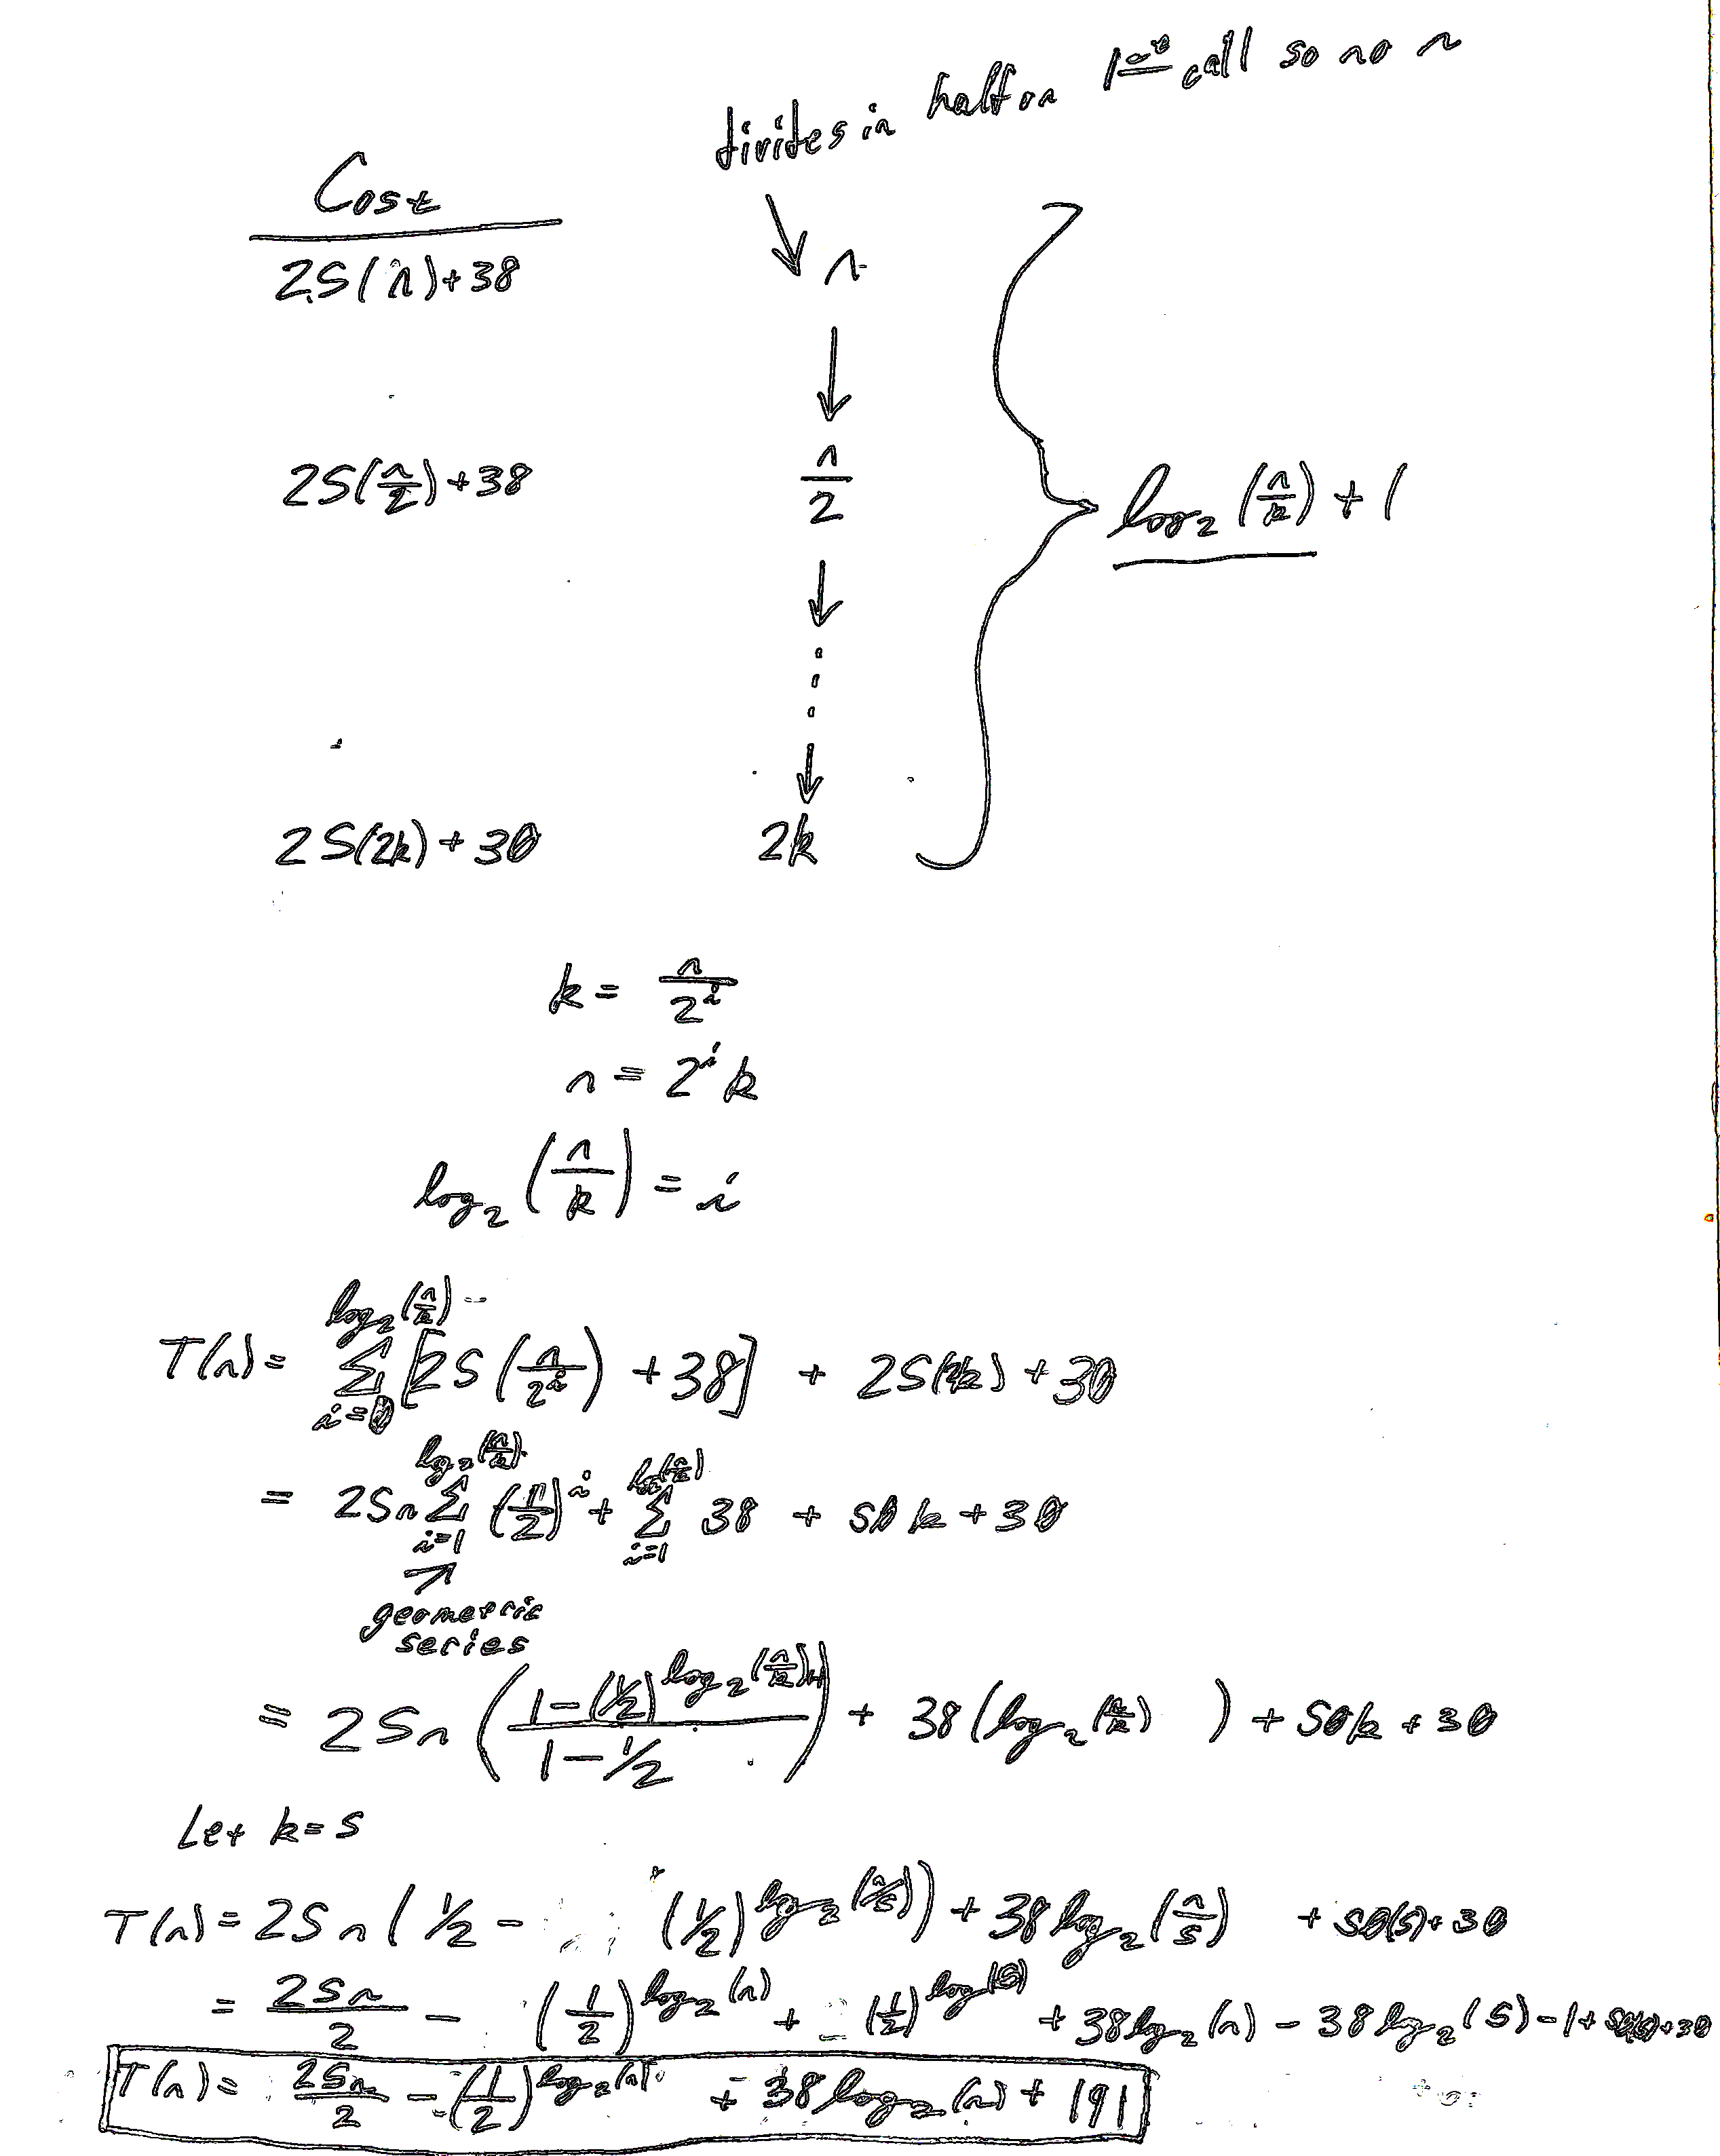
\includegraphics[width = \textwidth]{pics/alg4c}
  \end{figure}
\item
  Each algorithm to within some error matches its given
  graph. 

  Algorithm 1 matches on the slope well, but is off by a
  constant factor. However, this can be accounted for by system
  specific things such as stack and functional call time.

  Algorithm 2 has approximately the same slope as its real
  counterpart. The constant factor is within enough of an error bound
  to be a good approximation of the T(n).

  Algorithm 3 has approximately the same slope as its real
  counterpart. The theoretical complexity is faster than its real
  complexity; however, this can be accounted for by the system
  specifics such as multiple processes running. This is reasonable due
  to the main difference being in a constant factor over all.

  Algorithm 4 is the most markedly different between its real and
  theoretical T(n). This however is accounted for by its recursive
  nature. Any recursive algorithm will run slower than its theoretical
  due to system specifics such as stack frames and function
  calls. This explains the difference in slopes.
\item
  For the real running time of the algorithms, they were ordered least to
  most efficient: algorithm 1, algorithm 2, algorithm 4, algorithm 3.
\item
  For the theoretical running time of the algorithms, they were
  ordered least to most efficient: algorithm 1, algorithm 2, algorithm
  4, algorithm 3.
\item
  Yes, both the theoretical and real complexity of the algorithms lead
  to the same ordering of the algorithms based on efficiency. This is
  to be expected. The only slightly odd exception is that the
  recursive algorithm 4 theoretically stayed in the same order. This
  was because its theoretical efficieny is linear and with a smaller
  constant factor than algorithm 3. However, algorithm's 4 logrithmic
  term boosted to a slower rate than algorithm 3.
\end{enumerate}
\end{document}